\section{Reliability Mechanisms}
\label{sec:reliability}

The biggest risk in a long-horizon run is execution drift, not weak reasoning.
Argus therefore ships a set of guards that keep a mission bounded and honest ---
each one domain-agnostic, each one refusing to make a scientific judgment itself.
Figure~2 sketches how they wrap a single mission's engineer/reviewer loop.

\begin{figure}[t]
\centering
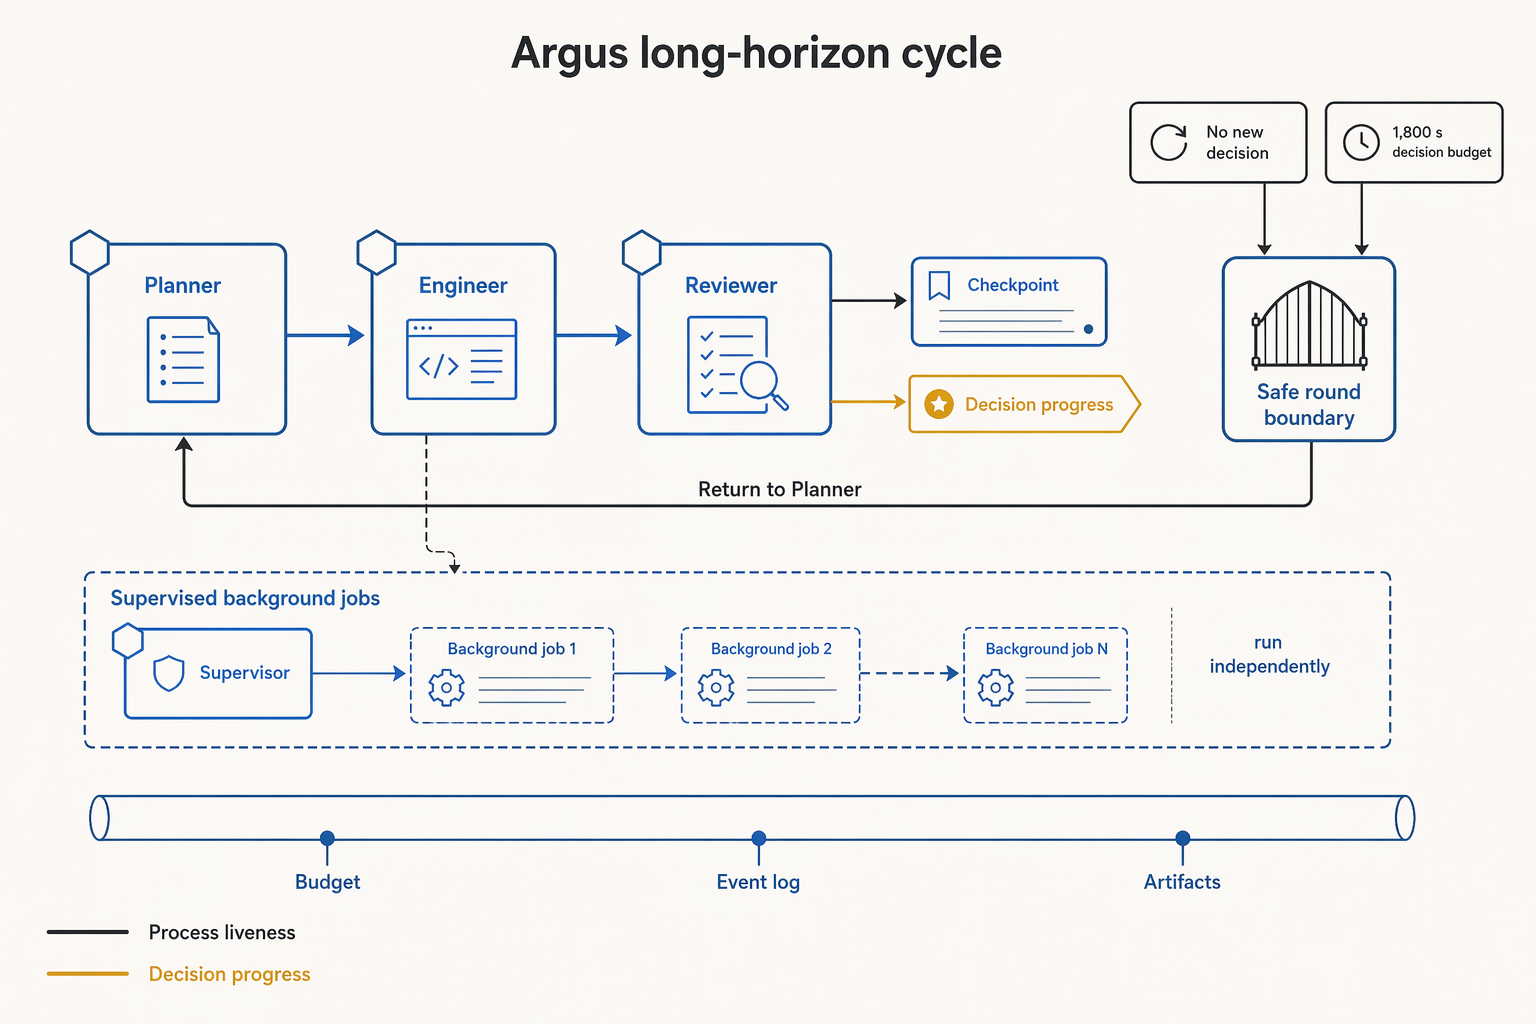
\includegraphics[width=0.82\textwidth]{figures/long_horizon_reliability.png}
\caption{System schematic (not a measured performance plot) of the Argus
long-horizon reliability cycle: Planner, Engineer, and Reviewer run one
continuous loop; the Reviewer emits a single bounded checkpoint and a
decision-progress class that reseeds a fresh Engineer thread; supervised
background jobs run independently alongside the loop; and a safe round
boundary returns a stalled or budget-exhausted mission to the Planner, all
on top of a persistent budget, event-log, and artifact rail.}
\label{fig:reliability}
\end{figure}

\subsection{Curated working-memory checkpoint}

A single mission's session is resumed round after round, and left unchecked it
grows into millions of tokens and is compacted lossily many times, erasing
working memory and driving the amnesia loop described in
Section~\ref{sec:introduction}. Argus fixes this without a watchdog. The Reviewer
--- acting as a memory auditor --- maintains a small, \emph{hard-capped}
checkpoint: goal, done items, tried-and-failed attempts, a ``maturing'' list for
promising-but-unproven directions, an open blocker, and the next step. The caps
are enforced in code, not merely requested in a prompt (for example, at most a
handful of done and tried items, each a short line), because the cap \emph{is} the
forgetting mechanism: deleting stale detail is the antidote, and the ground truth
always remains on disk in the artifacts. Each round the Engineer proposes a
handoff; the Reviewer validates it against evidence and writes the next canonical
checkpoint. The runner renders that checkpoint as a ``curated working memory''
block at the top of the next Engineer prompt. If the Reviewer ever mis-writes the
checkpoint, the runner keeps the previous one --- it never blanks memory.

\subsection{Bounded session roll}

The checkpoint is only half the fix; the session itself must stay short-lived. A
thread is proactively dropped and reseeded from the checkpoint into a
\emph{fresh} session after \textbf{3 consecutive rounds} (the default
\code{shift\_round\_limit}) \emph{or} once the previous round's input reaches
\textbf{1.5M tokens} (the default \code{thread\_token\_limit}). Both are
configurable through environment variables, and either can be disabled by setting
it to zero. The round-count roll bounds context within a single mission; the
token-count roll catches an inherited, already-bloated thread on its first round,
because a thread resumed across many short missions can reset the round counter
before it ever fires. With per-session context bounded, the runaway
hundred-compaction spiral cannot occur, and the existing context-pressure and
poisoned-session cleanup paths now reseed from the checkpoint --- rebirth rather
than amnesia.

\subsection{Structured decision-progress classification}

To distinguish real progress from busy churn, the Reviewer labels each round with
a \code{progress\_class}: \code{decision} or \code{evidence} (genuine forward
motion), or \code{setup\_only}, \code{artifact\_sync\_only}, or \code{none}
(nondecision work). The harness counts these structured labels; it never infers
progress from activity. \textbf{Two consecutive} nondecision rounds trip a stall
counter (the default \code{stall\_threshold}). This is paired with a safe
\textbf{1{,}800-second} round-boundary budget measured from the last decision or
evidence increment. The budget is checked only \emph{between} rounds --- it never
interrupts a live provider call --- so it can end a mission that is spinning
without ever severing useful in-flight work. A separate soft/hard round-limit
escalation catches the rarer case of a mission that makes evidence progress every
round but never passes its gate, asking the Reviewer to return \code{blocked} on an
external dependency and, failing that, force-ending as \code{blocked} so the
Planner re-plans.

\subsection{Dynamic review cadence}

Reviewing every round is the default, but it is occasionally wasteful: when the
Engineer has just landed a real increment and the next step is unambiguous, a
Reviewer round would only restate it. In that case the Engineer may append a
single \code{CONTINUE\_WORK: <next step>} line to request one deferred review. It
may defer only once in a row; the last available round always returns to the
Reviewer; and \code{done} can still come only from the Reviewer. The harness does
not guess from prose whether to skip --- it responds only to the explicit request.

\subsection{Background-subagent cadence wait}

When the Engineer starts a self-monitored long-running job --- a GPU training run
that already has its own supervisor checking health, early-stopping on failure,
and reporting a terminal result --- babysitting it every round wastes budget.
Argus reads the subagent registry and classifies in-flight jobs as
self-watched or needs-attention. If the Engineer explicitly replies
\code{WAIT\_FOR\_SUBAGENT: <task\_id>} and that id matches a healthy self-watched
job, the runner skips the expensive Reviewer round and sleeps on the job's own
monitoring cadence (clamped to a safe 30--900\,s), waking early when the job
finishes. The wait is the agent's explicit choice, not the harness deciding for
it; a stale or mismatched sentinel is simply ignored.

\subsection{Live credential guard}

Finally, a domain-agnostic secret guard scrubs newly written artifacts for
credentials before they reach the event log or the Reviewer's prompt, and redacts
persisted event and usage copies. Redaction never judges scientific quality; when
it rewrites an artifact it tells the Reviewer so provenance hashes can be rebuilt,
and a scan error or oversized artifact explicitly blocks unconditional
certification rather than silently passing.

\begin{callout}[A shared property of every guard]
None of these mechanisms decides whether the research is good. Each one enforces a
domain-agnostic invariant --- bounded context, counted decisions, a safe budget, a
supervised wait, a scrubbed artifact --- and every one fails soft, preserving the
agent's memory and judgment when anything goes wrong. That is the difference
between a harness that makes autonomy reliable and one that quietly takes the
science out of the agent's hands.
\end{callout}
